%\documentclass[a4paper]{article}
\documentclass[17pt]{extarticle}
\usepackage{polyglossia}
\usepackage{epigraph, varwidth}
\renewcommand{\epigraphsize}{\small}
\setlength{\epigraphwidth}{0.9\textwidth}
\usepackage{color, colortbl}
\usepackage{xcolor}
\usepackage{graphicx}
\usepackage{tabularx} % in the preamble
\usepackage[margin=15mm]{geometry}
\usepackage{hyperref}
\hypersetup{
    backref=true,
    citecolor=magenta,
    colorlinks=true,
    linkcolor=blue,
    filecolor=magenta,
    urlcolor=cyan,
}
\urlstyle{same}
\setmainfont[Scale=0.9]{Noto Serif}
\setotherlanguages{marathi}
\newfontfamily\marathifont[Mapping=velthuis-sanskrit,Script=Devanagari,Language=Marathi]{Noto Serif Devanagari}
% define acronyms https://tex.stackexchange.com/a/73681/64425
\usepackage{xspace}
\newcommand*{\subjmath}{Mathematics, Introduction to Proofs, and Problem-solving\xspace}
\newcommand*{\subjsci}{Introduction to Science (Focus on Chemistry)\xspace}
\newcommand*{\subjeng}{English (Grammar and Basic Composition)\xspace}
\newcommand*{\subjmusic}{\textmarathi{hi.mdusthaanii sa.mgiita - 1} (Indian Classical Music - 1)\xspace}
\newcommand*{\subjart}{Art and Craft}
% define acronyms https://tex.stackexchange.com/a/73681/64425
% control hyphenation: https://tex.stackexchange.com/a/177179/64425
\tolerance=1
\emergencystretch=\maxdimen
\hyphenpenalty=10000
\hbadness=10000
% control hyphenation: https://tex.stackexchange.com/a/177179/64425
% make sure ~ as non-breaking space doesn't interfere with velthuis-sanskrit mapping
\edef~{\string~}
\begin{document}
% ....
\begin{center}
\begin{minipage}{.4\textwidth}
%\centering
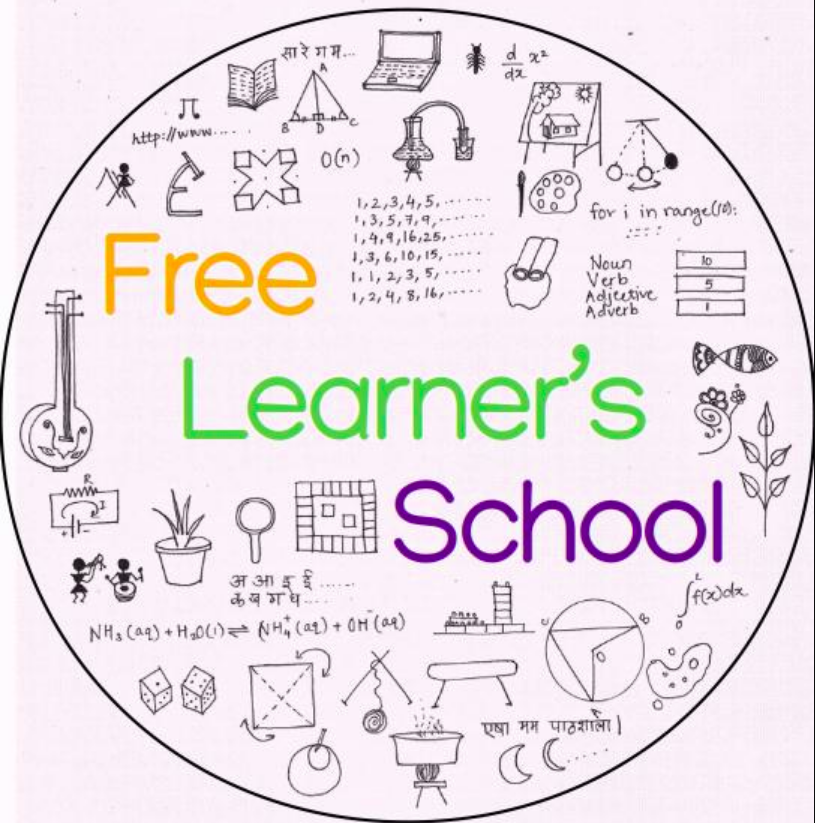
\includegraphics[height=2cm]{fls-school-logo.png}
\end{minipage}
\end{center}
\centering
{\Large \underline{Report Card}}
\begin{tabularx}{\textwidth}{lX}
Name: &  Rujuta Mhaswade\\
Grade: & Six \\
Academic Year: &2020-21  \\
\end{tabularx}
\vspace{10mm}
\begin{tabularx}{\textwidth}{|X|l|l|}
\hline
  \textbf{Subject} & \textbf{Instructor} & \textbf{Grade} \\
\hline
\subjmath &
Kedar Mhaswade&
\textcolor{magenta}{\textbf{A-}}
\\
\hline
\subjsci &
Kedar Mhaswade&
\textcolor{magenta}{\textbf{A-}}
\\
\hline
\subjeng&
Kedar Mhaswade&
\textcolor{magenta}{\textbf{A-}}
\\
\hline
\subjmusic&
Deepa Joshi and Kunda Joshi&
\textcolor{magenta}{\textbf{A}}
\\
\hline
\subjart &
Deepa Joshi &
    \textcolor{magenta}{\textbf{None!}}
\\
\hline
\end{tabularx}
\underline{Comments (With Constructive Feedback)}
\begin{enumerate}
\item \textbf{\subjmath}. Rujuta took great interest in math this year. We followed \textbf{Arithmetical Excursions} \cite{ae} which introduced some new concepts and reintroduced known concepts. She is now pretty comfortable with the Place-Value System in various positive integer bases, Operations on Integers, Axioms of Arithmetic like Commutative and Associative properties of Addition and Multiplication and Distributive property of Addition and Subtraction, the Long Division Algorithm, the Fundamental Theorem of Arithmetic (I still remember her excitement about the FTA and its use in the reduction of fractions), Laws of Exponentiation, Deductive Reasoning and the Notion of ``Proofs'' in Mathematics, Fractions, Large Numbers, and First Steps in Algebra. There is, of course, a lot to learn, but we think that she took great interest, solved problems, completed exercises, took notes, and enjoyed her time.

Perhaps she should focus a bit more on problem-solving. She is actually very tenacious and likes the challenge and excitement that problems pose. When we present a problem, she is more than excited to solve it, toil through the experience. Perhaps she should explore problems on her own. We tried NRICH problem sets \cite{nrich}, but she couldn't do it regularly. We urge her to take a look at problems and find patterns that make those problems. Of course, this is most enjoyable when it is done voluntarily.

Her term-end exam \cite{math-exam} was really difficult. She scored about $60\%$ in it and we are really proud of her. Though she was a bit disappointed by her performance in that exam, when we asked her if she wanted an ``easy exam with direct application of learned content'' or a ``tough exam with surprising twists and turns", she chose the latter. This means that she is here to learn and grow, rather than \emph{only} excel at examinations.

She also read ``Alice's Adventures in Wonderland'' and ``Through the Looking Glass'' \cite{aiw} with great interest and dedication. We are glad that she thoroughly enjoyed these books that are at the intersection of lasting literature and mathematics.

        For the next year, she should brush up what has been learned till now, look at where in the term-end examination she could have improved, and be as enthusiastic as ever to learn something new in a friendly environment.

\item \textbf{\subjsci}. Teaching Science to children is hard. The process of Science, like any other subject, starts with an interest in figuring out or understanding how things work. And, as such, it takes, among other things, curiosity, tenacity, imagination, skepticism, patience, and playful nature to learn and spend time well in Science.

We picked up Robert Brent's Golden Book of Chemistry Experiments \cite{golden} and came to know of the Scientific Method, the Periodic Table of Elements, Basic Properties of matter like Mass, Volume, and Density, Units and Measurements. We studied some chemical elements in some detail. We also looked at chemical equations and balancing reactions. We performed several experiments, most notable of which was the ``Electrolysis of Water''. Rujuta has maintained the lab of Chemistry very meticulously. We are really thankful to her for that!

        The Science term-end exam \cite{science-exam} was also tough and although we asked several thought-provoking questions, she fared well. We are proud of her result. We'll perhaps take up middle school chemistry \cite{middleschoolchemistry} (again) next year. She should brush up what we did last year before we start the next year.

\item \textbf{\subjeng}. We picked up Warriner's book for English Grammar \cite{warriner}. She became pretty comfortable with Grammar (including Parts of Speech, Prepositional Phrases, Complements, and Using Parts of Speech Correctly), Mechanics, and some Composition. We also read and reread some books like Alice in Wonderland \cite{aiw}, Stuart Little, and Charlotte's Web. Check out her notes \cite{english-notes} that have become really a dependable source for us as well!

She worked hard on the English term-end exam \cite{english-exam}. We are very satisfied with the result. She should, however, work more on her reading and creative writing. She should apply more in her own writing what she learned through the year. Writing well is very difficult and although we understand that

\epigraph {
Vigorous writing is concise. A sentence should contain no unnecessary words, a paragraph no unnecessary sentences, for the same reason that a drawing should have no unnecessary lines and a machine no unnecessary parts. This requires not that the writer make all sentences short or avoid all detail and treat subjects only in outline, but \textbf{that every word tell}.
}
{
  -- \textit{E. B. White}
}

, it is important to keep up the practice of writing. And it is hard to imagine writing more than reading. More books should be picked up in order to enjoy the writing process even more.
\item \textbf{\subjmusic}. Deepa Joshi taught her the basics of Indian Classical Music. Rujuta learned \textmarathi{ala.mkaara} (arrangement of some or all of the 7 fundamental frequencies: \textmarathi{saa, re, ga, ma, pa, dha, ni}) and six \textmarathi{raaga} (Ragas) in Indian Classical Music: \textmarathi{bhuupa} (Bhoop), \textmarathi{yamana} (Yaman), \textmarathi{durgaa} (Durga), \textmarathi{bhairava} (Bhairav), \textmarathi{baage"srii} (Bageshree), and \textmarathi{desa} (Des). In each \textmarathi{raaga}, she learned its basic rules - \textmarathi{aaroha} (Aroha), \textmarathi{avaroha} (Avaroha), and \textmarathi{paka.da} (Pakad). She learned a few signature vocal pieces (\textmarathi{ba.mdi"sa}) representing each \textmarathi{raaga}. She also learned to sing them in three different \textmarathi{taala} (rhythms) on the \textmarathi{tabalaa} (\emph{tablaa}) - \textmarathi{tiinataala} (Teentaal), \textmarathi{ekataala} (Ektaal), and \textmarathi{daadaraa} (Dadaraa). She can effectively use iTablaPro \cite{itp}, an amazing app for the iPhone, to set up referential frequencies and notes. One admirable thing is every once in a while she practices her music on her own; it has become a developing hobby for her!

See Mrs. Kunda Joshi's (an accomplished practitioner of Indian Classical Music and a great teacher of it) assessment (in Marathi) of Rujuta's Term-end exam performance in Figure \ref{fig: kbj-feedback}.
        \begin{figure}[h]
            \centering
            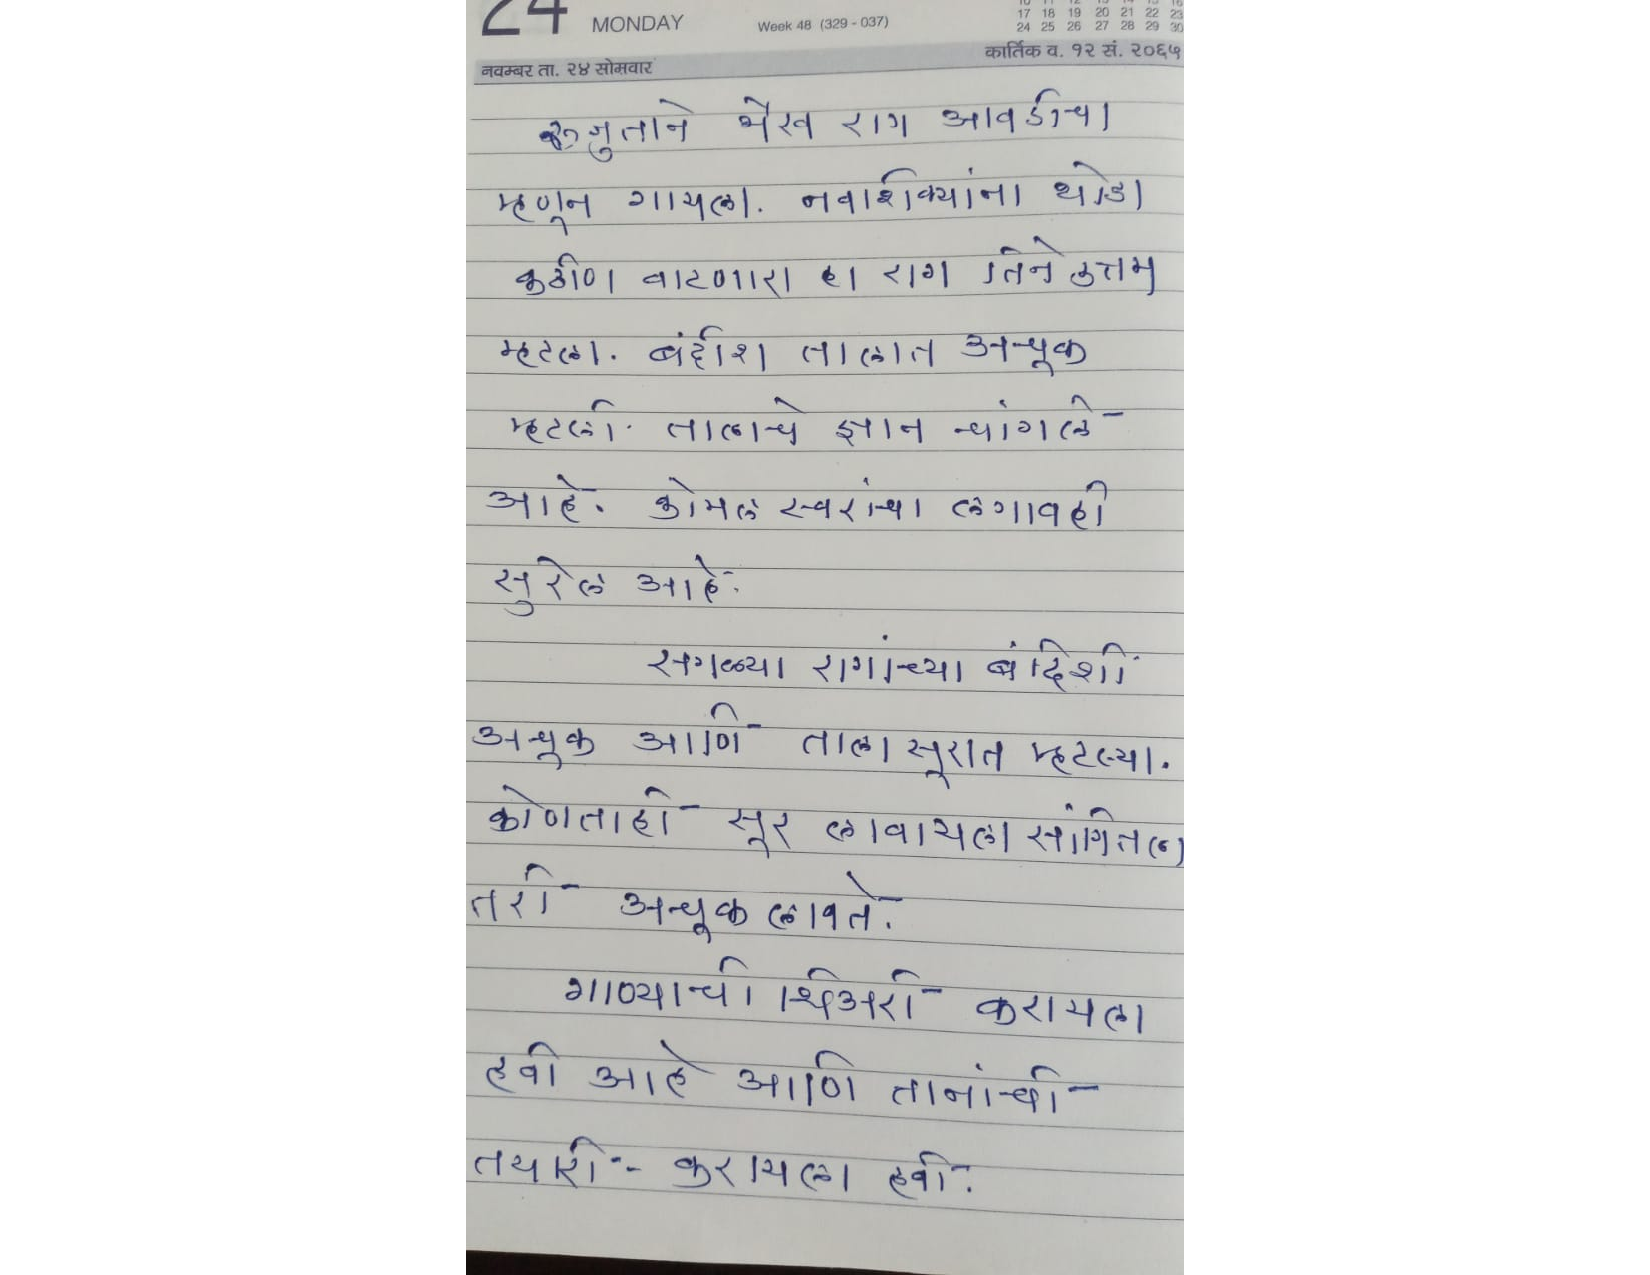
\includegraphics[width=1.0\linewidth]{rujuta-music-exam-1-feedback.pdf}
            \caption{Mrs. Kunda Joshi's Assessment of Rujuta's Performance}
            \label{fig: kbj-feedback}
        \end{figure}

We are encouraging her to appear for the \textmarathi{prave"sikaa prathama} (Entrance Exam: 1) exam of the well-known \href{https://abgmvm.org/}{\textmarathi{gaa.mdharva sa.mgiita mahaavidyaalaya} (Gaandharva music school)}.
\item \textbf{\subjart}. Rujuta created many rangolis this year. She recreated some of them on GeoGebra \cite{geogebra}. She also learnt about two Indian folk arts - \textmarathi{vaaralii} (Warli) and \textmarathi{madhubanii} (Madhubani). She showed some interest in \textmarathi{madhubanii} and we created five paintings together. Two of them were about two Indian festivals - \textmarathi{dasaraa} (Dasara) and \textmarathi{divaaLii} (Diwali). She worked really hard on those two paintings.
\end{enumerate}
\newpage
\begin{thebibliography}{00}
    \bibitem{ae} Henry Bowers, Joan E. Bowers. Arithmetical Excursions, An Enrichment of Elementary Mathematics. Dover Publications Inc. New York. Available to borrow digitally at \href{https://archive.org/details/arithmeticalexcu00bowe/page/n5/mode/2up}{archive.org}.
    \bibitem{nrich}  Innovative Collaboration between Mathematics Faculties and Education at the University of Cambridge. On the WWW at \href{https://nrich.maths.org/about}{nrich.maths.org}.
    \bibitem{math-exam}  Mathematics Term-end Exam 2021. Free Learner's School. Available at \href{https://github.com/kedarmhaswade/writings/blob/main/english/math/rujuta-term-end-math-exam-2021.pdf}{GitHub}.
    \bibitem{aiw} \href{https://en.wikipedia.org/wiki/The_Annotated_Alice}{Alice's Adventures in the Wonderland and Through the Looking Glass}. Lewis Carroll. Annotated by Martin Gardner. Clarkson N. Potter Publishers. 1960. 
    \bibitem{golden} \href{https://en.wikipedia.org/wiki/The_Golden_Book_of_Chemistry_Experiments}{The Golden Book of Chemistry Experiments}. Robert Brent. Illustrator: Harry Lazarus. Annotated by Martin Gardner. Clarkson N. Potter Publishers. 1960. 
    \bibitem{science-exam} Science Term-end Exam 2021. Free Learner's School. Available at \href{https://docs.google.com/document/d/1HZHNTQ3jDHIAhcJIuh7TvnkRdlJGYK1KEme9rVcpXec/edit?usp=sharing}{Google Docs}.
    \bibitem{middleschoolchemistry} Middle School Chemistry -- Big Ideas about the Very Small. Available at \href{https://www.middleschoolchemistry.com/download/}{ACS: Chemistry for Life}.
    \bibitem{warriner} English Grammar and Composition. John. E. Warriner and Harcourt Brace Jovanovich. Available to borrow digitally at \href{https://archive.org/details/englishgrammarco00holt}{archive.org}.
    \bibitem{english-exam} English Term-end Exam 2021. Free Learner's School. Available at \href{https://docs.google.com/document/d/1D6EzUiXNP7Yfh2hzVPXdeOOvV0HJWWFJHBvQDo3tjEA/edit}{Google Docs}.
    \bibitem{english-notes} Rujuta's Notes of Warriner's English. Free Learner's School. Available at \href{https://docs.google.com/document/d/198iSeBMoAQyS2hIIpjpDlzStoVtRBXMi6NnwRzOELNY/edit?usp=sharing}{Google Docs}.
    \bibitem{itp} iTablaPro iPhone App. Available at \href{https://apps.apple.com/in/app/itablapro/id337350026}{Apple App Store}.
    \bibitem{geogebra} GeoGebra graphic calculator. Available at \href{https://geogebra.com}{GeoGebra Website}.
\end{thebibliography}
\end{document}
